\documentclass{article}


%programs
\usepackage{amsmath, amssymb, amsthm, bbm} % Math environments
\usepackage{hyperref}                % Links
\usepackage{enumitem}                % Better lists
\usepackage{tcolorbox}               % Boxed environments for notes
\usepackage{geometry}                % Page layout
\usepackage{microtype} % Adjusts spacing and kerning for better readability
\usepackage{todonotes}


% shortcuts
\newcommand{\R}{\mathbb{R}} % For real numbers
\newcommand{\C}{\mathbf{C}} % For complex numbers

\newcommand{\E}{\mathbb{E}} % For expected value
\newcommand{\N}{\mathbb{N}} % For natural numbers
\newcommand{\prob}{\mathbb{P}} % For probability
\newcommand{\indf}{\mathbbm{1}} % indicator function
%structure theorem allowed
\newcommand{\threeprob}{(\Sigma, \mathcal{F}, \mathbb{P})} 



\newtheorem{theorem}{Theorem}[section] % Theorem numbering restarts in each section
\newtheorem{proposition}[theorem]{Proposition} % Propositions follow Theorem numbering
\newtheorem{lemma}[theorem]{Lemma} % Lemmas follow Theorem numbering
\newtheorem{corollary}[theorem]{Corollary} % Corollaries follow Theorem numbering

\theoremstyle{definition} % Change style for definitions and similar environments
\newtheorem{definition}{Definition}[section] % Definitions restart numbering in each section
\newtheorem{example}{Example}[section] % Examples restart numbering in each section
\newtheorem{remark}{Remark}[section] % Remarks restart numbering in each section

\geometry{margin=1in}                % Adjust margins


\title{Lecture Notes on Non-Parametric Econometrics}
\author{ETE spirit}
\date{These notes have been last updated on \today}


\begin{document}

\maketitle
\tableofcontents
\cleardoublepage

\section{Notes on Probability}

\subsection{On measure space}

Let \(\Sigma\) be a set, we want to make sense of $\mathbb{P}(F)$ the probability of the event F, where \(F\subseteq\Sigma\).



\begin{definition}
A collection of subsets of \(\Sigma\) is a \(\sigma\)-algebra if:
\begin{itemize}
    \item \(\Sigma \in F\)
    \item \( f \in F \implies F^{c}=\left\{w \in \Sigma : w \notin F\right\}\in F\)
    \item For every sequence \((F_{n})\) of elements of F, \(\bigcup_{n \in N}F_{n} \in F\). Note that this property is the same as: \(\bigcap_{n \in N}(F_{n}^{c})^{c}\) 
\end{itemize}
\end{definition}

\begin{remark}
    In measure theory, one axiomatizes the notion of 'measurable set', insisting that the union of a countable collection of measurable sets is measurable, and that the intersection of a countable collection of measurable sets is also measurable. Also, the complement of a measurable set must be mea- surable, and the whole space must be measurable. Thus the measurable sets form a sigma-algebra, a structure stable (or 'closed') under countably many set operations. Without the insistence that 'only countably many operations are allowed', measure theory would be self-contradictory - a point lost on certain philosophers of probability \footnote{straight copy pasting from the glorious and much helpful book "Probability with martingales" by Williams"}.
\end{remark}
\begin{example}
    If \(\Sigma=\mathbb{R}^{d}\), the Borel sigma-algebra, denoted \(\mathbb{B}(\mathbb{R}^{d})\) is the smallest sigma-algebra of \(\mathbb{R}^{d}\) which contains all open sets. 
\end{example}


\begin{definition}
    \(\mu: F \rightarrow [0, \infty]\) is a measure on \(\Sigma, F\) if: \begin{itemize}
        \item \(\mu(\emptyset)=0\)
        \item if for all sequences \((F_{n})_{n \in N}\) of disjoint sets of F we have that \(\mu(\bigcap)_{n \in N}=\sum_{n \in N}\mu(F_{n})\)
    \end{itemize}
\end{definition}

\begin{definition}
    $\mathbb{P}$ is a probability if it is a measure and  $\mathbb{P}(\Sigma)=1$
\end{definition}

\begin{definition}
    \((\Sigma, F, \mathbb{P})\) is a probability triple if $F$ is a sigma-algebra on $\Sigma$ and $\mathbb{R}$ a probability on \((\Sigma, F)\).
\end{definition}

\begin{definition}
\(X:(\Sigma, F, \mathbb{P})\rightarrow (\mathbb{R}^{d}, \mathbb{B}(\mathbb{R}^{d}))\) is a random vector if \(\forall \mathbb{B} \in \mathbb{B}(\mathbb{R}^{d}) , X^{-1}(\mathbb{B} \in F) \). That is, X is f-measurable. 
\end{definition}

\begin{example}
    \textbf{Measurability of a Random Variable: A Simple Example}
    
    Let us consider a sample space \(\Omega = \{HH, HT, TH, TT\}\), representing the outcomes of flipping a fair coin twice. Define a random variable \(X: \Omega \to \{0, 1, 2\}\), which takes the following values based on the number of heads in the outcome:
    \[
    X(\omega) = \begin{cases} 
    0 & \text{if } \omega = TT, \\
    1 & \text{if } \omega = HT \text{ or } \omega = TH, \\
    2 & \text{if } \omega = HH.
    \end{cases}
    \]
    
    To determine whether \(X\) is measurable with respect to a given \(\sigma\)-algebra \(\mathcal{F}\), recall that measurability means for every Borel set \(B \subseteq \{0, 1, 2\}\), the preimage \(X^{-1}(B) = \{\omega \in \Omega : X(\omega) \in B\}\) must belong to \(\mathcal{F}\).
    
    
    Suppose \(\mathcal{H}\) is the trivial \(\sigma\)-algebra \(\{\emptyset, \Omega\}\). For example, consider the preimage \(\{X = 2\} = \{HH\}\). Clearly, \(\{HH\} \notin \mathcal{H}\), so \(X\) is not \(\mathcal{H}\)-measurable.
    
Define a \(\sigma\)-algebra \(\mathcal{F}\) where \(X\) is measurable
    Now, let us construct a \(\sigma\)-algebra \(\mathcal{F}\) such that \(X\) is measurable. Consider the following \(\sigma\)-algebra:
    \[
    \mathcal{F} = \{\emptyset, \Omega, \{HH\}, \{TH, HT\}, \{TT\}, \{HH, TT\}, \{TH, HT, TT\}, \{HH, TH, HT\}\}.
    \]
    
    We verify that \(\mathcal{F}\) is a \(\sigma\)-algebra (it is closed under complements and countable unions). Next, we check whether \(X\) is measurable with respect to \(\mathcal{F}\).\\
    
   
    We calculate the preimages of the sets \(\{0\}\), \(\{1\}\), and \(\{2\}\):
    \[
    \{X = 0\} = \{TT\} \in \mathcal{F},
    \]
    \[
    \{X = 1\} = \{HT, TH\} \in \mathcal{F},
    \]
    \[
    \{X = 2\} = \{HH\} \in \mathcal{F}.
    \]
    Since the preimages of all singleton sets in the range of \(X\) belong to \(\mathcal{F}\), and \(\sigma\)-algebras are closed under unions, the preimages of all Borel subsets of \(\{0, 1, 2\}\) also belong to \(\mathcal{F}\). Therefore, \(X\) is \(\mathcal{F}\)-measurable. \\

    \end{example}
    
\begin{definition}
    Let X be a random vector in $\mathbb{R}^{d}$, the sigma-algebra generated by X, denoted $\sigma(X)$ is the smallest sigma-algebra on $\Sigma$ s.t: \(X:(\Sigma, F, \mathbb{P})\rightarrow (\mathbb{R}^{d}, \mathbb{B}(\mathbb{R}^{d}))\) is measurable.
\end{definition}

\begin{example}
    Consider a probability space \((\Sigma, \mathcal{F}, \mathbb{P})\) where:
    \begin{itemize}
        \item \(\Sigma = \{a, b, c\}\),
        \item \(\mathcal{F} = \{\emptyset, \{a\}, \{b, c\}, \{a, b, c\}\}\),
        \item \(\mathbb{P}(\{a\}) = 0.5\), \(\mathbb{P}(\{b, c\}) = 0.5\).
    \end{itemize}
    Define a random variable \(X : \Sigma \to \mathbb{R}^2\) as:
    \[
    X(a) = (1, 2), \quad X(b) = (3, 4), \quad X(c) = (5, 6).
    \]
    We claim \(X\) is measurable. To see why, consider any Borel set \(B \in \mathbb{B}(\mathbb{R}^2)\):
    \begin{itemize}
        \item If \(B = \{(1, 2)\}\), then \(X^{-1}(B) = \{a\} \in \mathcal{F}\).
        \item If \(B = \{(3, 4), (5, 6)\}\), then \(X^{-1}(B) = \{b, c\} \in \mathcal{F}\).
        \item If \(B = \mathbb{R}^2\), then \(X^{-1}(B) = \{a, b, c\} \in \mathcal{F}\).
    \end{itemize}
    Since \(X^{-1}(B) \in \mathcal{F}\) for all \(B \in \mathbb{B}(\mathbb{R}^2)\), \(X\) is measurable. This demonstrates how random variables map events in the sample space to measurable subsets of \(\mathbb{R}^2\).
    \end{example}


\begin{remark}
    \begin{itemize}
        \item  \(x \in \mathbb{R}^{d} \rightarrow [0, \infty)\)
        \item \(x \mapsto \|x\|_{2}^{\rho}, \text{ where } \rho > 1 
        \quad \left( 
        \|x\|_{2} = \sqrt{\sum_{k=1}^{d} x_k^2} 
        \right)\) is continuous, as a consequence we can show that \( \|x\|_{2}^{\rho}\) is a random variable if X is a random vector \textbf{Exercise 1}
    \end{itemize}
\end{remark}

\begin{definition}
    We write \(X \in L^{\rho}(\Sigma, F, \mathbb{P})\) if X is F-measurable and \(\mathbb{E}[\|x\|^{\rho}_{2}]< \infty\)
\end{definition}

\begin{definition}
The distribution law of X, denoted $\mathbb{P}_{x}$ is the probability on $(\mathbb{R}^{d}, \mathbb{B}(\mathbb{R}^{d}))$ such that \(\forall \mathbb{B} \in \mathbb{B}(\mathbb{R}^{d})\), \(\mathbb{P}(X \in \mathbb{B})= \mathbb{P}_{x}(\mathbb{B})\)
\end{definition}

\begin{definition}
    X has density \(f_{x}\) with respect to the Lebesque measure $(dx)$ on \(\mathbb{R}\) if \(\prob_{x}(B)=\int_{\R^{d}} \indf \left\{x \in B\right\} f_{x} dx , \forall B \in \mathbb{B}(\R^{d})\), where \(f_{x} dx\) is \(d\prob_{x}(x)\)
\end{definition}

\begin{definition}
    The support of X (or of $\prob_{x}$) is defined as: \(\text{Supp(X)}=\left\{x \in \R^{d} : \forall r>0, \prob(X \in B(X,r))>0\right\}\) where \(B(x,r):=\left\{z:\|x-z\|_{2}<r\right\}\) is an open ball. 
\end{definition}

\begin{remark}
    \begin{itemize}
        \item \(\text{Supp(X)}^{c}:=\left\{x \in \R^{d} : \forall r>0, \prob(X \in B(X,r))=0\right\}\) is an open set and hence the Supp(X) is a closed set. 
        \item Supp(X) is the longest? \(C \in \mathbb{B}(\R^{d})\) such that for all ball B such that \(B \cap C \neq \emptyset \implies \prob_{x}(B \cap C )>0\)
    \end{itemize}
\end{remark}

\textbf{Exercise:} let \(Y= Y^{*} \indf \left\{Y^{*} \geq \frac{1}{2}\right\}+ \frac{1}{3} \indf \left\{Y^{*} < \frac{1}{2}\right\}\) show that: \begin{enumerate}
    \item \(supp(Y^*)=[-1,1] \)
    \item \(supp(Y)=\frac{1}{3} \cup [\frac{1}{2},1]\)
\end{enumerate}

\begin{remark}
    Note that: \(\E[|y|]\leq \sqrt{\E(y^{2})}\) by Cauchy-Schwarz so \(L^{2}(\Sigma, \mathcal{F}, \mathbb{P})\), where we can define: \(\E(|y|)=\E(Y \cdot sign(Y))\).
\end{remark}

\textbf{Exercise:} If X is a random vector and $X_{1}$ the rth entry, then \(\sigma(X_{1})\subset \sigma(X)\)

\subsection{Conditional probability}

\begin{definition}
    For a random variable \( X \in L^1(\Omega, \mathcal{F}, P) \), we define the \emph{expectation} \(\mathbb{E}(X)\) of \(X\) by
    \[
    \mathbb{E}(X) := \int_\Omega X \, dP = \int_\Omega X(\omega) P(d\omega).
    \]
    We also define \(\mathbb{E}(X) \leq \infty\) for \(X \in (\mathcal{mF})^+ \). In short, \(\mathbb{E}(X) = P(X)\).
    \end{definition}


\begin{definition}
    Let \(Y \in L^{1}(\threeprob)\) and X be a random vector in $\R^{d}$. We define \(z:=\E[Y|X]\) is the unique\footnote{unique means that if z and z' satisfy 1 and 2 $\implies z=z' a.s$} random v then: 
    \begin{itemize}
        \item \(z \in L^{1}(\Sigma, \sigma(x), \prob)\), where z is both integrable and $\sigma$-x-measurable. 
        \item \(\forall B \in \mathbb{B}(\R^{d}) \E(z \cdot \indf\left\{x\in B\right\})=\E(y \cdot \indf\left\{x\in B\right\})\)
        \item The second condition is true \(\iff \E((y-z) \cdot \indf \left\{x\in B\right\})=0 \iff \E((y-z) \cdot \Phi(x))\)
    \end{itemize}
\end{definition}


\begin{remark}
    \(z\) is \(\sigma(x)\) measurable \(\iff z=\varphi(x)\) for some \(\varphi_{i}(\R^{d}, \mathbb{B}(\R^{d}))\rightarrow (\R^{d}, \mathbb{B}(\R^{d}))\), which in words it means that z is a function of x which in turn is measurable. 
\end{remark}

Another definition we can find it in the book: 

\begin{definition}[Fundamental Theorem and Definition (Kolmogorov, 1933)]
    Let \((\Omega, \mathcal{F}, P)\) be a triple, and \(X\) a random variable with \(\mathbb{E}(|X|) < \infty\). Let \(\mathcal{G}\) be a sub-\(\sigma\)-algebra of \(\mathcal{F}\). Then there exists a random variable \(Y\) such that:
    \begin{enumerate}
        \item \(Y\) is \(\mathcal{G}\)-measurable,
        \item \(\mathbb{E}(|Y|) < \infty\),
        \item for every set \(G \in \mathcal{G}\) (equivalently, for every set \(G\) in some \(\pi\)-system which contains \(\Omega\) and generates \(\mathcal{G}\)), we have
        \[
        \int_G Y \, dP = \int_G X \, dP, \quad \forall G \in \mathcal{G}.
        \]
    \end{enumerate}
    Moreover, if \(\tilde{Y}\) is another random variable with these properties, then \(\tilde{Y} = Y\), a.s., that is, \(P[\tilde{Y} = Y] = 1\). A random variable \(Y\) with properties \((a)-(c)\) is called a version of the  \(\mathbb{E}(X \mid \mathcal{G})\) of \(X\) given \(\mathcal{G}\), and we write \(Y = \mathbb{E}(X \mid \mathcal{G})\), a.s.
    \end{definition}
    

\begin{remark}
    There are two particular cases: \begin{enumerate}
        \item \((y,x')'\) with discrete countable support, the definition then coincides with: \(\E(Y|X=x)=\sum_{y_{j}\in \text{supp}_{y}}y_{j}\cdot \prob(Y=y_{j}|X=x)\). If x is such that \(\P(X=x)>0\).
        \item \((y,x')'\) and X have a density then \( \E(y|X=x)=\int_{\R}y \cdot \frac{\mathcal{f}_{y,x}(y,x)}{\mathcal{f}_{x}(x)}dy\)
    \end{enumerate}
\end{remark}

\textbf{exercise} Let X and B be random vectors in $\R^{d}$ such that X and B are independent. Let \(g: \R^{d} \mapsto \R\) be continuous and bounded and \(Y=g(x_{i}'B_{i})\), show that then \(\E[Y|X=x]=\E[x_{i}'B_{i}] \forall x \in
\text{supp}(X)\)

\textbf{Exercise: provide the proof of this properties.}
\subsubsection{Some properties of the conditional expectation function}
Note: the idea of the proof of this properties can be found in pages 88 and 89 of the masterful book Probailities with martingales. The development and errors are due only to myself. 
\begin{enumerate}
    \item Let \(Y\in L^{1}(\threeprob)\)\footnote{we assume this throughout this exercise} then \(\E[\E[y|x]]=\E[y]\). 
    
    \begin{proof}
    By the definition of conditional expectation, \(\E[Y|X]\) satisfies:
    \[
    \int_A \E[Y|X] \, d\mathbb{P} = \int_A Y \, d\mathbb{P}, \quad \forall A \in \sigma(X).
    \]
    Setting \(A = \Omega\), we have:
    \[
    \int_\Omega \E[Y|X] \, d\mathbb{P} = \int_\Omega Y \, d\mathbb{P}.
    \]
    The left-hand side is \(\E[\E[Y|X]]\), and the right-hand side is \(\E[Y]\). Thus, we conclude:
    \[
    \E[\E[Y|X]] = \E[Y].
    \]
    \end{proof}
    \item Let \(g(\R^{d}, \mathbb{B}(R^{d}))\rightarrow (\R^{d}, \mathbb{B}(R^{d}))\) measurable such that \(\E[g(x)]<\infty\) then \(\E[g(x)|x]=g(x) a.s\). 
    
    \begin{proof}
        From Remark 1.5, we know that a random variable \(Z\) is \(\sigma(X)\)-measurable if and only if \(Z = \varphi(X)\) for some measurable function \(\varphi : (\mathbb{R}^d, \mathbb{B}(\mathbb{R}^d)) \to (\mathbb{R}^d, \mathbb{B}(\mathbb{R}^d))\). 
        
        Let \(Z = g(X)\). By assumption, \(g\) is measurable and \(\E[|g(X)|] < \infty\), so \(Z\) is \(\sigma(X)\)-measurable. 
        
        It is a property of conditional expectation that if \(Z\) is \(\sigma(X)\)-measurable and \(\E[|Z|] < \infty\), then \(\E[Z|X] = Z\) almost surely. Applying this property to \(Z = g(X)\), we conclude:
        \[
        \E[g(X) | X] = g(X) \quad \text{a.s.}
        \]
        \end{proof}




    \item \(\forall a_{1}, a_{2} \in \R\) and \(\E[|Y_{1}|+|Y_{2}|]<\infty\) then \(\E[a_{1}Y_{1}+a_{2}Y_{2}]=a_{1}E[Y_{1}]+a_{2}[Y_{2}] a.s\)
    \begin{proof}
        Given that \(\E[|Y_{1}| + |Y_{2}|] < \infty\), the random variables \(Y_1\) and \(Y_2\) are integrable, and their conditional expectations are well-defined. Consider the random variable \(a_1 Y_1 + a_2 Y_2\). By the definition of conditional expectation, we have:
        \[
        \E[a_1 Y_1 + a_2 Y_2 | X] = \int_A (a_1 Y_1 + a_2 Y_2) \, d\mathbb{P},
        \]
        for all \(A \in \sigma(X)\).
        
        Using the linearity of the integral, this can be expressed as:
        \[
        \int_A (a_1 Y_1 + a_2 Y_2) \, d\mathbb{P} = \int_A a_1 Y_1 \, d\mathbb{P} + \int_A a_2 Y_2 \, d\mathbb{P}.
        \]
        
        Taking the constants \(a_1\) and \(a_2\) outside their respective integrals, we get:
        \[
        \E[a_1 Y_1 + a_2 Y_2 | X] = a_1 \int_A Y_1 \, d\mathbb{P} + a_2 \int_A Y_2 \, d\mathbb{P}.
        \]
        
        By the definition of conditional expectation, this becomes:
        \[
        \E[a_1 Y_1 + a_2 Y_2 | X] = a_1 \E[Y_1 | X] + a_2 \E[Y_2 | X].
        \]
        
        Thus, the result follows:
        \[
        \E[a_1 Y_1 + a_2 Y_2 | X] = a_1 \E[Y_1 | X] + a_2 \E[Y_2 | X] \quad \text{a.s.}
        \]
        \end{proof}
        




    \item if \(y\geq 0\) a.s then \(\E[Y|X]\geq0\) a.s.
    
    \begin{proof}
        Let \(Z = \E[Y | X]\). Suppose \(\mathbb{P}(Z < 0) > 0\). Then there exists \(G := \{Z < -n^{-1}\}\) for some \(n \in \mathbb{N}\) with \(\mathbb{P}(G) > 0\) and \(G \in \sigma(X)\). By the definition of conditional expectation:
        \[
        \int_G Y \, d\mathbb{P} = \int_G Z \, d\mathbb{P}.
        \]
        Since \(Y \geq 0\) a.s., \(\int_G Y \, d\mathbb{P} \geq 0\), but \(\int_G Z \, d\mathbb{P} < -n^{-1} \mathbb{P}(G) < 0\)\footnote{Since \(Z(\omega) \leq -n^{-1}\) for all \(\omega \in G\), it follows that \(Z(\omega) \leq -n^{-1}\) on \(G\). Therefore, the integral satisfies:
        \[
        \int_G Z \, d\mathbb{P} \leq \int_G (-n^{-1}) \, d\mathbb{P} = -n^{-1} \mathbb{P}(G).
        \]}, a contradiction. Thus, \(\mathbb{P}(Z < 0) = 0\), so \(Z \geq 0\) a.s.
        \end{proof}
        
        



    \item Let \(c:\R\rightarrow \R\) be a convex function such that \(\E[|c(y)|]<\infty\) then \(\E[c(y)|x]\geq c[\E[y|x]]\) a.s.
    
    We will use the following definition - which requires that function c is continuous (6.6.a in Williams): \( c(x)=sup_{q\in G}\left[D_{-c}(q)(x-q)+c(q)\right]=sup_{n}(a_{n}x + b_{n})\) for some sequences in $a_n b_n \in \R$\footnote{The definition expresses \( c(x) \) as the supremum of affine functions \( a_n x + b_n \) for sequences \( a_n \) and \( b_n \), which correspond to the subgradients \( D_{-c}(q_n) \) and values \( c(q_n) \) at points \( q_n \). This means that \( c(x) \) can be constructed as the pointwise upper bound of all linear approximations of the function based on its subgradients at various points. Intuitively, each linear function \( a_n x + b_n \) is a "supporting hyperplane" to the convex function at a specific point, and the supremum ensures that \( c(x) \) is the tightest convex function that satisfies these inequalities.}.

    \begin{proof}
        If we apply this definition to this problem we know that \(c(x)=sup_{n}(a_n x + b_n)\) and \(c(x)\geq (a_n x + b_n)\) for a fixed  $n \in \N$. Then we take expectations in both sides:  \(\E(c(x)|\zeta)\geq (a_n \E(x|\zeta) + b_n)\), where $\zeta \in \sigma(x)$. Then for all n, this is also true by countability property\footnote{The countability property allows the supremum over all \(n \in \mathbb{N}\) to replace the fixed \(n\) case, ensuring the inequality applies to the entire sequence.}
        : \(\E(c(x)|\zeta)\geq sup_n(a_n \E(x|\zeta) + b_n)=c(\E(x|\zeta))\). 
    \end{proof}

    \(\)




    \item Let \(\mathcal{H}, \xi\) be the sigma-algebra and that \(\mathcal{H}\subset \xi\). Then \(\E[\E[y|\xi]|\mathcal{H}]=\E[Y|\mathcal{H}]\) a.s.
    
    \begin{proof}
        By the definition of conditional expectation, \(\mathbb{E}[Y|\xi]\) satisfies \(\int_A \mathbb{E}[Y|\xi] \, d\mathbb{P} = \int_A Y \, d\mathbb{P}\) for all \(A \in \xi\).  
        Now consider \(\mathbb{E}[\mathbb{E}[Y|\xi]|\mathcal{H}]\). By the definition of conditional expectation, for any \(B \in \mathcal{H}\),
        \[
        \int_B \mathbb{E}[\mathbb{E}[Y|\xi]|\mathcal{H}] \, d\mathbb{P} = \int_B \mathbb{E}[Y|\xi] \, d\mathbb{P}.
        \]
        Since \(\mathcal{H} \subset \xi\), every \(B \in \mathcal{H}\) is also in \(\xi\), so we have
        \[
        \int_B \mathbb{E}[Y|\xi] \, d\mathbb{P} = \int_B Y \, d\mathbb{P}.
        \]
        Thus, by the uniqueness of conditional expectation, \(\mathbb{E}[\mathbb{E}[Y|\xi]|\mathcal{H}] = \mathbb{E}[Y|\mathcal{H}]\) almost surely.
        \end{proof}


    \item Let z be a bounded random variable (i.e \(\exists M \in \R : |z|\leq M a.s\)) that is y measurable. Then \(\E[zy|\xi]=z\E[y|\xi]\) a.s. \footnote{\textbf{this is taken from the glorious book that was recommended in class}}
    
    \begin{proof}
        Fix \(G \in \xi\) and let \(W = \mathbb{E}[Y|\xi]\). We aim to prove that
        \[
        \mathbb{E}[ZY \mid G] = \mathbb{E}[Z \cdot W \mid G].
        \]
        
        If \(Z\) is the indicator function of a set \(A \in \xi\), then by the definition of conditional expectation, the result holds:
        \[
        \mathbb{E}[\mathbf{1}_A Y \mid G] = \mathbf{1}_A \mathbb{E}[Y \mid G].
        \]
        
        Linearity of the conditional expectation implies that the result holds for any simple function \(Z \in SF^+(\Omega, \xi, \mathbb{P})\). By the monotone convergence theorem\footnote{ \(if X_n\geq 0\) then if  \( \E(X_n|\zeta)\) increases, \(\E(X_n|\zeta)\) also increases.}, the result extends to non-negative, \(\xi\)-measurable random variables. Finally, for a general bounded \(\xi\)-measurable random variable \(Z\), we decompose \(Z\) into positive and negative parts and apply linearity (proof given above). Thus, the property is proven.
        \end{proof}



\end{enumerate}

\begin{remark}
    If \(z\in L^{p}(\Sigma, \xi, \prob)\) and \(y\in L^{q}(\threeprob)\) where \(\xi \subset \Sigma\) and \(\frac{1}{p} + \frac{1}{q}=1\) and \(p,q\geq1\) then \(\E[zy|\xi]=z\E[y|\xi]\) a.s. 

    This is an application of the \textbf{Hühler inequality}, which is defined as follows: \(\E[|zy|]\leq \E[|z|^{p}]^{\frac{1}{p}}\E[|y|^{q}]^{\frac{1}{q}} \) and this is defined \(\forall p,q\geq 0 : \frac{1}{p} + \frac{1}{q}=1\)\footnote{when p=q=2 this is the Cauchy-Schwarz inequality.}
\end{remark}


\subsection{Some notes on identification (from lecture 2)}
Data consists of draws from \(\prob_{y,x}\) where y and x are vectors that are observed by the econometrician. X is determined outside the model. \textbf{A structural econometrics model} consists of: \begin{enumerate}
    \item An equation \(v(y, \gamma, X, \epsilon; \zeta )=0\) where v is a vector of functions, \(\gamma\) is a vector of unobserved variables determined inside the model, \(\epsilon\) unobserved variables determined outside the model and \(\zeta\) which corresponds vector's function distribution??? \textbf{check notes because this makes little sense to me}
    \item Restriction: \(\zeta \in \mathcal{R}\): for example, then our draw would be \(\prob_{y,x;\zeta}\) is the distribution of observables generated by \(\zeta\). 
\end{enumerate} 


\begin{example}
    \begin{enumerate}
        \item \( Y = f(X) + \varepsilon \), where \( \Sigma = \{f, P_{X}, \varepsilon\} \). This is a type of regression.
        \item \( \mathbb{E}(|f(X)| + |\varepsilon|) < \infty \), and \( \mathbb{E}[\varepsilon \mid X] = 0 \), with \(f\) continuous on \(\text{supp}(X)\).
    
        In this case, we have:
        \[
        \mathbb{E}[Y \mid X] = \mathbb{E}[f(X) \mid X] + \mathbb{E}[\varepsilon \mid X] = f(X),
        \]
        where \(f\) is the conditional expectation function (i.e., the regression function).
    \end{enumerate}
    \end{example}
    
    \begin{example}
    \begin{enumerate}
        \item \( Y = f(X) + \varepsilon \), where \( \Sigma = \{f, P_{X,Z,\varepsilon}\} \), and the distribution of the observed data is \( P_{Y,X,Z} \). Here, \( Z \) is determined outside the model.
        \item \( \mathbb{E}(|f(X)| + |\varepsilon|) < \infty \), \( \mathbb{E}[\varepsilon \mid Z] = 0 \), and \(f\) is continuous on \(\text{supp}(X)\), with additional restrictions.
    \end{enumerate}
    \end{example}
    
    \begin{example}
        We have these two equations:
        \begin{enumerate}
            \item \( Y_1 = \alpha_{12} Y_2 + g_1(X_1) + \varepsilon_1 \),
            \item \( Y_2 = \alpha_{21} Y_1 + g_2(X_2) + \varepsilon_2 \),
            
        \end{enumerate}
        where:
            \[
            X = \begin{pmatrix} X_1 \\ X_2 \end{pmatrix}, \quad 
            \varepsilon = \begin{pmatrix} \varepsilon_1 \\ \varepsilon_2 \end{pmatrix}, \quad
            Y = \begin{pmatrix} Y_1 \\ Y_2 \end{pmatrix},
            \]
            and \(\alpha_{12}, \alpha_{21} \in \mathbb{R}\), while \(g_1\) and \(g_2\) are unknown functions.
            
            The model can be written as:
            \[
            \gamma(Y, \gamma, X, \varepsilon, \zeta) = 0,
            \]
            where \(\zeta = \begin{pmatrix} \alpha_{12} \\ \alpha_{21} \\ g_1 \\ g_2 \\P_{X, \varepsilon} \end{pmatrix}\) and explicitly:
            \[
            \gamma = 
            \begin{pmatrix} 
            \alpha_{12} Y_2 + g_1(X_1) + \varepsilon_1 - Y_1 \\
            \alpha_{21} Y_1 + g_2(X_2) + \varepsilon_2 - Y_2
            \end{pmatrix}=0
            \]

        \textbf{Case 2}: If \(\alpha_{12}\) and \(\alpha_{21}\) are random, then we can assume \(\varepsilon \) satisfies one of the following restrictions:
        \[
        \mathbb{E}[\varepsilon \mid X] = 0, \quad \mathbb{E}[\Sigma \mid X] = 0, \quad \text{or} \quad \varepsilon \perp X.
        \]
            And now the parameters are  where \(\zeta = \begin{pmatrix}  g_1 \\ g_2 \\P_{X, \varepsilon} \end{pmatrix} \quad \varepsilon=\begin{pmatrix}
            a_{12} \\ g_{21} \\  \varepsilon_1 \\\varepsilon_2
            \end{pmatrix}\)

        \textbf{Case 3}: If \(\gamma = \begin{pmatrix} \alpha_{12} \\ \alpha_{21} \end{pmatrix}\), we can be in a setup where the distribution of the observed data is \(P_{Y, X, Z}\) and the assumptions \(Z \perp Y\) hold in R.
    \end{example}


    \begin{example}
        This is an example of non-parametric IV that was used by the professor, with not much success, to introduce and convey in us a passion for the assumption of completeness:

\begin{enumerate}
    \item \(Y_{1}=f(x)+\epsilon\) and the distribution of the observed data is \(\prob_{y,x,z}\). We are interested in $\varphi=f$.
    \item Restrictions: \begin{itemize}
        \item \(f\) is continuous on the \(supp(x)\).
        \item \(\E\left[|f(x)|+|\epsilon|\right]<\infty\)
        \item \(\E[\epsilon|z]=0\)
        \item \textbf{Completeness}: if $\varphi$ is continuous in the \(supp(x)\) s.t \(\E |\varphi(x)|<\infty\) then \(\E(\varphi(x)|z)=0 \implies x\in \text{supp}(x), \varphi(x)=0 \). 
    \end{itemize}
\end{enumerate}
    \end{example}


    \begin{example}
        \textbf{Exercise 4.1} \((x', z')'\) has a finite support such that supp(x)=\(\left\{x_{1}, \cdots, x_{k}\right\}\) and supp(z)=\(\left\{z_{1}, \cdots, z_{l}\right\}\) then show that \(\E\left[\varphi(x)|z=z_{l}\right]=0\). \\
        We can define \(\E\left[\varphi(x)|z=z_{l}\right]=\sum_{k=1}^{k}\varphi(x_{k})\prob \left(x=x_{k}|z=z_{l}\right)\). This is equal to 0 iff \(\varphi \cdot M_{k,l}=0\), we can apply the rank theorem\footnote{\(\dim \ker(\mu) + \text{rank}(\mu)=k\)} to show that this holds only if the k vector $\varphi$ is equal to 0. \\

    \textbf{Exercise 4.2}
In this exercise we are interested in finding a sufficient condition under which completeness holds. \textbf{To complete in another occasion}

    \end{example}


    \begin{example}
Let \(x, \beta\) be two random variables in \(\R^{d}\) s.t \(x \perp \beta\). Let \(g:\R^{d} \rightarrow \R\) be continuous and bounded. We define \(y=g(x'\beta)\), we need to show that \(\E(y|X=x)=\E[g(x'\beta)]\). For simplicity we define $\varphi(x)=g(x'\beta)$. The argument needs to proof these two points: 
\begin{enumerate}
    \item $\varphi(x) \in L^{1}(\threeprob)$. The function is $x$-measurable.
    \item Let \(B \in \mathbb{B}(\mathbb{R}^{d})\), then \(\mathbb{E} \left[y \mathbf{1} \left\{x \in B \right\}\right] = \mathbb{E} \left[\mathbb{E} \left[ g(x'\beta) \right] \mathbf{1} \left\{x \in B \right\}\right]\).
\end{enumerate}

 
    
    To verify the first point, by definition:
    \[
    \varphi(x) = \int_{\mathbb{R}^{d}} g(x'\beta) \, d\mathbb{P}_{\beta}(b).
    \]
    Since \(g\) is continuous and bounded, \(g(x'\beta)\) is continuous as a function of \(x\). The integral of a continuous function over \(\beta\) is also continuous in \(x\). This implies that \(\varphi(x)\) is a continuous function of \(x\), and thus \(\varphi^{-1}(C)\) is in \(\mathbb{B}(\mathbb{R}^{d})\). Hence, \(\varphi(x)\) is measurable. \\
    
    For the second part, consider \(\mathbb{E}_{x, \beta}[g(x'\beta) \indf \{x \in B\}]\), where \(B \in \mathbb{B}(\mathbb{R}^{d})\). By the definition of joint expectation:
    \[
    \mathbb{E}[g(x'\beta) \indf \{x \in B\}] = \int_{\mathbb{R}^{d}} \int_{\mathbb{R}^{d}} g(x'\beta) \indf \{x \in B\} \, d\mathbb{P}_{x}(x) \, d\mathbb{P}_{\beta}(b).
    \] 
    
    Here, the independence of \(x\) and \(\beta\) plays a critical role. Independence implies that the joint probability measure \(d\mathbb{P}_{x, \beta}(x, b)\) can be written as \(d\mathbb{P}_{x}(x) \cdot d\mathbb{P}_{\beta}(b)\). This factorization allows us to separate the expectation as:
    \[
    \int_{\mathbb{R}^{d}} \int_{\mathbb{R}^{d}} g(x'\beta) \indf \{x \in B\} \, d\mathbb{P}_{x}(x) \, d\mathbb{P}_{\beta}(b).
    \]

    
    Using Fubini’s theorem\footnote{This step is valid because the integrand \(g(x'\beta) \indf \{x \in B\}\) is bounded and the measures \(\mathbb{P}_x\) and \(\mathbb{P}_\beta\) are finite.}, we can swap the order of integration:
    \[
    \int_{\mathbb{R}^{d}} \int_{\mathbb{R}^{d}} g(x'\beta) \indf \{x \in B\} \, d\mathbb{P}_{\beta}(b) \, d\mathbb{P}_{x}(x).
    \]

    The inner integral depends only on \(\beta\), and the outer integral captures the expectation over \(x\).The outer integral then accounts for the distribution of \(x\), weighted by \(\indf \{x \in B\}\)
    
    By evaluating the inner integral, it follows that:
    \[
    \mathbb{E}[g(x'\beta) \indf \{x \in B\}] = \mathbb{E}[\mathbb{E}[g(x'\beta)] \indf \{x \in B\}],
    \]
 
    
    which completes the proof.
    \end{example}
    
    
    \subsubsection{Definitions of Identification}

We often care about \( \Psi^* = \Psi(\zeta) \) for a certain \(\Psi : \mathcal{R} \to \zeta\).

\begin{remark}
    \(\Gamma_{Y, X}(\Psi, \mathcal{R}) = \left\{ P_{Y, X, \zeta} \mid \zeta \in \mathcal{R}, \, \Psi(\zeta) = \Psi^* \right\}.
    \) It is the set of all distributions of the observables generated by \(\zeta\) consistent with \(\mathcal{R}\) and \(\Psi\).   

\end{remark} 

\begin{definition}
    Let \(\Psi, \Psi' \in \zeta\). \(\Psi\) and \(\Psi'\) are directionally equivalent if:
    \(
    \Gamma_{Y, X}(\Psi, \mathcal{R}) \cap \Gamma_{Y, X}(\Psi', \mathcal{R}) \neq \emptyset.
    \)
      
\end{definition}


\begin{definition}
   \(\Psi^*\) is identified in model \((\mathcal{R})\) if:
\[
\forall \Psi \in \zeta, \quad \Gamma_{Y, X}(\Psi, \mathcal{R}) \cap \Gamma_{Y, X}(\Psi^*, \mathcal{R}) \neq \emptyset \implies \Psi = \Psi^*.
\] 
\end{definition}

\subsubsection{Completeness (from class 4)}

Supose $(x,z)$ has a density and we define \(x=x-\eta\) where \(z \perp \eta\) and $z$ and $\eta$ have densities. We may think of x as miss-measured. Completeness in this situation can be defined as: \(\forall \varphi\) continuou such that \(\forall z \in \R\): \[\int f_{\eta}(z-x)\varphi(x) dx=0 \implies \forall x \ \varphi(x)=0\]. 

\begin{example}
    \textbf{Example (Economic Context):} 

Suppose we are interested in estimating a structural model where the true relationship is:
\[
y = \beta x + \epsilon,
\]
but the observed covariate \(z = x + \eta\) is a mismeasured version of \(x\), where \(\eta\) represents classical measurement error. Here, \(z\) is the observed variable, and \(x\) and \(\eta\) are unobserved. To identify \(\beta\), we often rely on an instrumental variable \(w\) that satisfies the following conditions:
1. \(w \perp \epsilon\) (instrument exogeneity),
2. \(w \not\perp x\) (relevance),
3. \(w \perp \eta\) (independence from the measurement error).

Completeness plays a role in ensuring that \(x\) can be uniquely identified from the joint distribution of \((z, w)\). Specifically, the completeness assumption can be formulated as follows:

Let \(\varphi(x)\) be any measurable function such that:
\[
\mathbb{E}[\varphi(x) \mid z, w] = 0 \quad \text{a.s.}
\]
Completeness implies that \(\varphi(x) = 0\) almost surely. This ensures that no non-trivial function of \(x\) is orthogonal to all functions of \((z, w)\), thereby allowing \(x\) to be fully recovered from the observed data \((z, w)\). \\

\textbf{Why is this important?} 

Without completeness, the conditional expectation \(\mathbb{E}[y \mid z, w]\) might not provide unique information about \(x\), leading to non-identification of the structural parameter \(\beta\). Completeness guarantees that the instrument \(w\) and the observed covariate \(z\) together contain enough information to uniquely identify the true signal \(x\).\\

\textbf{Connection to Measurement Error:} 

In the classical measurement error setting, we have:
\[
z = x + \eta,
\]
where \(\eta \perp x\). The density \(f_\eta(z - x)\) "smooths out" the true \(x\), making it harder to identify without additional information (e.g., from an IV). Completeness ensures that the mapping \(M: \varphi \mapsto \big( z \mapsto \int f_\eta(z - x) \varphi(x) dx \big)\) is injective, preventing loss of information about \(x\). \\




\end{example}

\begin{remark}
    Completeness \(\iff\) M is injective, where \(M: \varphi \mapsto x \mapsto \int f_{\eta}(z-x)\varphi(x) dx \). \(f\) is injective if \(f(x)=f(y) \implies x=y\). If f is linear, checking \(f(0)=0\) is enough to check $f(x)=0 \implies x=0$ 
\end{remark}

\begin{remark}
    What is the density of \(z+ \eta\) when \(z \perp \eta\) and z and $\eta$ have a density? Let \(B \in \mathbb{B}(\R)\) then \(\prob(z+\eta)\in B= \int_{\R^{2}} \indf \left( z+\epsilon \in B \right) d\prob_{z,\eta}\), which by independence assumption is the same as: \(\int_{\R^{2}} \indf \left( z+\epsilon \in B \right) f_{z}(z)f_{\eta}(\eta) dz d\eta \). If we let \(u=z+\epsilon\) then we can express this integral as: \(\int_{\R^{2}} \indf \left( u\in B \right) f_{\eta}(u-z)f_{z}(z) du dz \) where we have also applied Fubini to reverse the order of integration. Finally, we can rewrite the last expression as this: \(\int_{\R^{2}} \indf \left( u\in B \right) int_{\R^{2}} f_{\eta}(u-z)f_{z}(z) dz du \) where  \(int_{\R^{2}} f_{\eta}(u-z)f_{z}(z)= f_{z+\eta}(u)\) by definition. 
\end{remark}

\begin{definition}
    \textbf{Characteristic Function:} 
    The characteristic function of a random vector \(x\) is defined as:
    \[
    \phi_x(t) = \E\left[\exp(i t'x)\right],
    \]
    where \(i^2 = -1\) and \(\exp(it) = \cos(t) + i \sin(t)\).
\end{definition}

Applying the characteristic function to the previous exercise, we find:
\[
\E\left[\exp(it(z + \eta))\right] = \E\left[\exp(itz)\right] \cdot \E\left[\exp(it\eta)\right],
\]
because \(z\) and \(\eta\) are independent. This simplifies a potentially complex integral into a product of two simpler terms, making it significantly easier to work with.

The characteristic function is useful because it relates expectations to the underlying distributions. Specifically:
\[
\E\left[\exp(itx)\right] = \E\left[\exp(itz)\right] \varphi(t).
\]
This allows us to estimate:
\[
\E[\exp(itz)] = \frac{\hat{\exp}(itx)}{\hat{\varphi}(t)}.
\]

This relationship demonstrates how characteristic functions can simplify inference problems, particularly when working with convolution or noisy data.

\textbf{Note:} This is the last example where convolution and characteristic functions are specifically useful in our econometric applications.

\begin{example}
    Consider the following model:
    \begin{enumerate}
        \item \(y_i = x_i'\beta_i + \epsilon_i,\)
        \item \(x_i \perp (\beta_i', \epsilon_i).\)
    \end{enumerate}
    
    One feature of interest in this model is \(f_{\beta_i}\), the distribution of \(\beta_i\) (e.g., to study the distributional effects of a treatment). The distribution \(f_{\beta_i}\) can be expressed as:
    \[
    f_{\beta_i} = \int_{\mathbb{R}^{d-1}} f_\beta(b) \, db_2 \cdots db_d,
    \]
    where \(d\) is the dimension of \(\beta_i\).

    Alternatively, this distribution can be estimated using the characteristic function. For a given \(t \in \mathbb{R}\), we have:
    \[
    \E\left[\exp(itx) \mid X = x\right] = \E\left[\exp\big(i(\beta'tx + t\epsilon)\big)\right].
    \]
    This equality follows because \(\E\left[\exp(itx) \mid X = x\right]\) is the characteristic function of \((\beta', \epsilon)'\) evaluated at \((tx, t)\).

    \textbf{Exercise:} As a suggested exercise, prove the equality above. Hint: Consider how the independence assumption \(x_i \perp (\beta_i', \epsilon_i)\) simplifies the decomposition of the expectation. Good luck!
    
    
\end{example}

\begin{definition}
    \(L^{p}(\R^{d})=\left(\text{measurable functions from}\ (\R^{d}, B(\R^{d})) \ \text{to} \ (\R, B(\R))\right): \int_{\R^{d}}|f(x)|dx <\infty\)
\end{definition}

\begin{remark}
    we can also have the following mapping: \((\R^{d}, B(\R^{d}))\mapsto (\C, B(\C))\)
\end{remark}

\begin{definition}
    If \(f \in L^{1} (\R^{d})\) the Fourier transform of f \(F[f]\) is obtained as \(\forall \omega \in \R^{d}\), \(F(f)(\omega)= \int_{\R^{d}}\exp(iw'x)f(x)dx\).
\end{definition}

\begin{definition}
    If $f$ and $g$ belong to $L^{1}(\R^{d})$, then the \textbf{convolution} of f g, denoted \((f * g)(z)=\int_{\R^{d}}f(x)g(z-x)dx\).  
\end{definition}

\begin{remark}
    The previous expression is also equal to \(\int_{\R^{d}}f(z-x)g(x)dx\) by change of variables. 
\end{remark}

\begin{proposition}
    If f and g belong to \(L^{1} (\R^{d})\implies (f * g)(z) \in L^{1} (\R^{d})\) and \(F[f * g](\omega)=F[f](\omega) F[g](\omega)\)
\end{proposition}

\begin{proposition}
    if f belong to \(L^{1} (\R^{d})\implies F[f]\) is continuous at \(\lim_{||\omega||_{2}\rightarrow \infty} F(f)(\omega)=0\)
\end{proposition}


\begin{example}
    \textbf{Gaussian Kernel: }let \(k(x)=\frac{1}{\sqrt{2\pi}}\exp \left(-\frac{x^{2}}{2}\right)\) then given that \(k \in L^{1}(\R^{d})\) and \(F[k](\omega)=exp \left(-\frac{\omega^{2}}{2}\right)\) is positive
\end{example}
 

\begin{example}
    \textbf{Box function: }Let \(k(x)=\frac{1}{2} \indf[|x|\leq1]\) then if \(k \in L^{1}\) and \(F[k](\omega)=\frac{1}{2}\int_{-1}^{1} \cos(wx) dx + \frac{i}{2}\int_{-1}^{1}sin(wx) dx\). Where the second integral is 0 and so this becomes: \(\frac{1}{2\omega}\left[sin(wx)\right]^{1}_{-1}\). 
\end{example}

\subsubsection{Properties of the Fourier transform}
Suppose \(f\) and \(F[f]\) belong to \(L^{1}\) and to \(L^{2}\)\footnote{Important to notice that if we talk about r.v then if \(x \in L^{2}\subseteq L^{1}\). This does not apply to functions belonging in \(L^{1}\).}. Then, the following properties apply: \begin{enumerate}
    \item \textbf{Plancherel equality: }\(\frac{1}{(2\pi)^{d}}||F(f)||^{2}_{2}=||f||^{2}_{2}\) by Cauchy-Schwarz. 
    \item \textbf{Fourier's inversion formula: }\(\forall x \in \R^{d}\), \(f(x)=\frac{1}{(2\pi)^{d}} F\left[[F(f)](-x)\right]=\frac{1}{(2\pi)^{d}}\int_{\R^{d}}e^{-iw'x}F[f](w)dw\)
\end{enumerate}

\subsection{class 5}
Some more notes to motivate completeness, as a titanic effort made by the professor to generate some enthusiasm in class. 

\begin{proposition}
    Let \(\varphi\) be a continuous function such that \(\varphi \in L^{1}\), \(x=z-\eta\), \(z \perp \eta\), and we assume that \(\eta\) has a density. Then \(\forall z \in \R \ \int_{\R}\varphi(x)f_{\eta}(z-x)dx=0 \implies \forall x \in \R \ \varphi(x)=0\). \\  
    
    This result shows that the interaction between \(\varphi(x)\) and \(f_\eta(x)\) vanishes entirely for all \(z\). The convolution integral being zero everywhere implies that \(\varphi(x)\) has no "effect" in the domain, forcing it to be identically zero. Completeness ensures no non-zero \(\varphi(x)\) can "hide" under such conditions.\\

    Also, \( \int_{\R}\varphi(x)f_{\eta}(z-x)dx=0 \implies F[\varphi](\omega) F[f_{\eta}](\omega)=F[0]=0 \ \forall \omega \) by properties of the Fourier transform defined above. \\
    
    By the convolution theorem, the Fourier transform of the convolution is the product of the transforms. If this product is zero, and \(F[f_\eta](\omega) \neq 0\), then \(F[\varphi](\omega)\) must be zero for all \(\omega\). This directly implies \(\varphi(x)\) is zero everywhere, given the Fourier transform uniquely determines a function.
\end{proposition}

\begin{example}
    \(f_{\eta}\) is the density of a mean-zero random variable. Then \([f_{\eta}](\omega)>0 \ \forall \omega\). \\
    
    The Fourier transform of a mean-zero density does not vanish anywhere, ensuring that any \(\varphi(x)\) convolved with \(f_\eta(x)\) will reflect entirely in the product \(F[\varphi](\omega) F[f_\eta](\omega)\). If \(F[\varphi](\omega) = 0\), this enforces that \(\varphi(x)\) is zero everywhere. \\

    This implies that \( \forall \omega \ F[\varphi](\omega)=0 \implies F[\varphi]=0\). So \(\varphi'=0\) almost everywhere. But given that \(\varphi(x)\) is continuous, then \(\varphi(x)=0\).
\end{example}

\begin{example}
    \(F[f_{\eta}](w)=\frac{\sin(w)}{w}\), \(\forall \omega \in \R\). Here we also have that \(\eta \sim U[-1,1]\). 
    
    Intuition: For the uniform distribution on \([-1, 1]\), the Fourier transform \(F[f_\eta](\omega)\) has zeros at \(\omega = k\pi\) for \(k \in \mathbb{Z} \setminus \{0\}\), corresponding to points where \(\sin(w) = 0\).

    Let \(\zeta=\left[f_{k}, k\in \mathbb{Z}\right]\) be the set of zeros of \(F[f_{\eta}]\). Then by the second property of the previous theorem, \(\forall \omega \in \R \diagdown \zeta\), \(F[\varphi](w)=0\). \\ 
    
    Outside the zeros of \(F[f_\eta](\omega)\), the Fourier transform forces \(F[\varphi](\omega) = 0\). Continuity of \(F[\varphi](\omega)\) ensures this behavior extends across all \(\omega\). \\

    Or, similarly, let \(\omega=k\pi\) for some \(h \in \mathbb{Z}\) and \((\omega_{n})_{n \in \N}\) a sequence in \(\R \diagdown \zeta\) such that \(\omega_n \rightarrow \omega\). Because \(F[\varphi]\) is continuous, then \(\lim_{n\rightarrow \infty}F[\varphi](\omega_n)=F[\varphi](\omega)\). Hence \(\forall \omega \ F[\varphi]=0\), and we can conclude using a similar argument as before that \(\varphi(x)=0\). \\

    This shows that the zeros of \(F[f_\eta]\) do not allow \(\varphi(x)\) to escape the conclusion of being identically zero. Continuity bridges gaps at points of zero, solidifying the result.
\end{example}

\clearpage
\section{Non-Parametric Estimation}

\subsection{Density estimation (Lebesgue)}
Let \(x_{1},...,x_{n}\) be identically distributed random variables. Imagine we want to estimate the density \(f_x\) of \(x\) which we assume to lie in a large class of densities.

\begin{example}
    \begin{enumerate} We have two examples: \\
        \item Densities such that \(\forall x, x'\in \R\), \(|f_{x}(x)-f_{x}(x')| \geq L|x-x'|\) for a certain \(L>0\). 
        \item Densities which are monothically increasing on \([0,1]\)
    \end{enumerate}
\end{example}

A nonparametric estimator is the histogram. Assume \(f_x : [0,1]\mapsto \R\) and divide \([0,1]\) into non-overlapping intervals that we denote \((A_j)_{j=1}^{m}\) of length h. We define \(n_{j}= \sum_{i=1}^{n}\indf \{\ X_i\in A_j \}\ \). Then the histogram estimator is just \(f_{x}(x)=\sum_{j=1}^{m} \frac{n_j}{n\cdot h} \indf \{\ x\in A_j \}\ \) which depends on $h$ (we want the smaller h as possible...). Then we also have this expression: \(f_{x}(x)=\sum_{j=1}^{m} \frac{n_j}{n\cdot h} \indf \{\ x\in A_j \}\ = \frac{1}{n\cdot h}\sum_{i=1}^{n} \sum_{j=1}^{m}  \indf \{\ x_{i} \in A_j ; X \in A_j \}\ \) \\

\begin{definition} \textbf{Kernel Density estimator}
    Let \(K \in L^{1}(\R)\) s.t \( \int_{\R}K(u) du=1\) and \(\hat{f}_{x}(x)=\frac{1}{nh}\sum_{i=1}^{m}K \left(\frac{X_{i}-x}{h}\right)\) is called a kernel density estimator with kernel $K$ and bandwidth $h$.\footnote{
        Some examples of Kernels are given in the class notes, but are omitted here for brevity. }
\end{definition}

\begin{example}
    We can start with an estimator of the CDF. Let's for example define \(F_x\) of $x$ as \(F_{x}(x)= \E[\indf \{\ X_i \leq x \}\ ] \), then \( \hat{F}_{x}(x)= \frac{1}{n} \sum_{i=1}^{n}\indf \{\ X_i \leq x \}\ \). We define $f_x$ as the pdf. \(\hat{f}_{x}(x)=\frac{\hat{F}_{x}\left(x+\frac{h}{2}\right)-\hat{F}_{x}\left(x-\frac{h}{2}\right)}{h}\) for a given $h>0$. This is equal to this expression: \(\frac{1}{nh}\sum_{i=1}^{n} \indf \left\{\ x-\frac{h}{2}<X_i \leq x+\frac{h}{2} \right\}\ \). This function is a generalization of the Rosenblatt estimator. For example, we have the following expression: 
\end{example}

\begin{remark}
    If we take expectation of the Kernel function we have the following expression: \(\E(\hat{f}_{x}(x))= \frac{1}{hn}\sum_{i = 1}^n \E \left(\left( \frac{x_i-x}{h}\right)\right)= \frac{1}{h} \E \left(k \left( \frac{x_i-x}{h}\right)\right)  = \frac{1}{h}\int_{\R}\left( \frac{y-x}{h}\right) f_{x}(y) dy\)
\end{remark}

\subsubsection{Mean squared error of kernel estimators}

\textbf{This definition is taken directly from the book by Tsybakov}
A basic measure of the accuracy of estimator $\hat{p}_n$ is its \textit{mean squared risk} (or \textit{mean squared error}) at an arbitrary fixed point $x_0 \in \mathbb{R}$:

\[
\text{MSE} = \text{MSE}(x_0) \triangleq \mathbb{E}_p \left[ \left( \hat{p}_n(x_0) - p(x_0) \right)^2 \right].
\]

Here, MSE stands for “mean squared error” and $\mathbb{E}_p$ denotes the expectation with respect to the distribution of $(X_1, \dots, X_n)$:

\[
\mathbb{E}_p \left[ \left( \hat{p}_n(x_0) - p(x_0) \right)^2 \right] \triangleq \int \cdots \int \left( \hat{p}_n(x_0, x_1, \dots, x_n) - p(x_0) \right)^2 \prod_{i=1}^n \left[ p(x_i) dx_i \right].
\]

We have 

\[
\text{MSE} = b^2(x_0) + \sigma^2(x_0)
\tag{1.4}
\]

where\footnote{this is found by plugging in \(\E(\hat{f}_n)\) inside the first equations and developing.}

\[
b(x_0) = \mathbb{E}_p[\hat{p}_n(x_0)] - p(x_0)
\]

and 

\[
\sigma^2(x_0) = \mathbb{E}_p \left[ \left( \hat{p}_n(x_0) - \mathbb{E}_p[\hat{p}_n(x_0)] \right)^2 \right].
\]

\begin{definition}
    \textit{The quantities $b(x_0)$ and $\sigma^2(x_0)$ are called the bias and the variance of the estimator $\hat{p}_n$ at a point $x_0$, respectively.}

\end{definition}

\textit{The quantities $b(x_0)$ and $\sigma^2(x_0)$ are called the bias and the variance of the estimator $\hat{p}_n$ at a point $x_0$, respectively.}

We will develop here the same reasoning that was developed in the TD. \\

\textbf{Bounds of the bias}

We have the following expression for the bias:

\[
b(x_0) = \mathbb{E}\left(\hat{f}'_n(x_0)\right) - f'(x_0).
\]

Using the definition of the kernel estimator, we write:

\[
b(x_0) = \mathbb{E}\left[-\frac{1}{n h^2} \sum_{i=1}^n k'\left(\frac{x_i - x_0}{h}\right)\right] - f'(x_0).
\]

Since the observations \( x_i \) are i.i.d., the expression simplifies to:

\[
b(x_0) = -\frac{1}{h^2} \mathbb{E}\left[k'\left(\frac{x_i - x_0}{h}\right)\right] - f'(x_0).
\]

Now, applying the definition of expectation, we have:

\[
b(x_0) = \int_{\mathbb{R}} -\frac{1}{h^2} k'\left(\frac{z - x_0}{h}\right) f(z) \, dz - f'(x_0).
\]

Using integration by parts for the term \(\int_{\mathbb{R}} k'\left(\frac{z - x_0}{h}\right) f(z) \, dz\), we recall the integration by parts formula:

\[
\int u \, dv = uv \Big|_{-\infty}^{+\infty} - \int v \, du,
\]

and set: \( u = f(z) \), so \( du = f'(z) \, dz \), \( dv = k'\left(\frac{z - x_0}{h}\right) \, dz \), so \( v = k\left(\frac{z - x_0}{h}\right) \cdot \frac{1}{h} \). \\

Thus, the integral becomes:

\[
\int_{\mathbb{R}} k'\left(\frac{z - x_0}{h}\right) f(z) \, dz = \left[f(z) \cdot k\left(\frac{z - x_0}{h}\right) \cdot \frac{1}{h}\right]_{-\infty}^{+\infty} - \int_{\mathbb{R}} k\left(\frac{z - x_0}{h}\right) \cdot \frac{1}{h} f'(z) \, dz.
\]

Substituting this result back:

\[
b(x_0) = -\frac{1}{h^2} \cdot h \cdot f(z) \cdot k\left(\frac{z - x_0}{h}\right) \Big|_{-\infty}^{+\infty} + \frac{1}{h^2} \cdot h \int_{\mathbb{R}} k\left(\frac{z - x_0}{h}\right) f'(z) \, dz - f'(x_0).
\]

The first term vanishes because the kernel \( k \) and the function \( f(z) \) are assumed to decay sufficiently fast at infinity (they are integrable), i.e.,

\[
\lim_{z \to \pm\infty} f(z) \cdot k\left(\frac{z - x_0}{h}\right) = 0.
\]

Thus, the bias simplifies to:

\[
b(x_0) = \frac{1}{h^2} \cdot h \int_{\mathbb{R}} k'\left(\frac{z - x_0}{h}\right) f'(z) \, dz - f'(x_0).
\]

Now we define \(\mu = \frac{z - x_0}{h}\), so that \(z = \mu h + x_0\) and \(dz = h \cdot d\mu\). Replacing these in the previous expression, we obtain:

\[
b(x_0) = \frac{1}{n} \int_{\mathbb{R}} h \cdot k(\mu) \cdot f'(\mu h + x_0) \, d\mu - f'(x_0).
\]

By assumption, f is l-time differentiable. Hence, we can use the $(l-1)$ Taylor expansion for \(f'(\mu h + x_0)\) around \(x_0\), we write:

\[
f'(\mu h + x_0) = f'(x_0) + f''(x_0) \mu h + \frac{f'''(x_0)}{2!} (\mu h)^2 + \cdots + \frac{f^{(l)}(x_0 + \tau \mu h)}{(l-1)!} (\mu h)^{l-1},
\]

where \(\tau \in (0, 1)\). Substituting this expansion into the integral gives:

\[
b(x_0) = \int_{\mathbb{R}} k(\mu) \left[f'(x_0) + f''(x_0) \mu h + \frac{f'''(x_0)}{2!} (\mu h)^2 + \cdots + \frac{f^{(l)}(x_0 + \tau \mu h)}{(l-1)!} (\mu h)^{l-1} \right] d\mu - f'(x_0).
\]

Using the property of the kernel function that \(\int_{\mathbb{R}} \mu^s k(\mu) \, d\mu = 0\) for all \(s = 1, \dots, l-1\) (where \(l\) is the order of the kernel), we simplify the expression to:

\[
b(x_0) = \int_{\mathbb{R}} k(\mu) \cdot \frac{f^{(l)}(x_0 + \tau \mu h)}{(l-1)!} (\mu h)^{l-1} \, d\mu.
\]

Now we introduce the Hölder condition for the function \(f\), which holds by assumption. A function \(f\) belongs to the Hölder class of order \((l)\) if:

\[
|f^{(l)}(x) - f^{(l)}(x')| \leq L |x - x'|^{\beta - l},
\]

which conveys that the norm is bounded and provides information on the smoothness of the function. Using this, we write:

\[
b(x_0) = \int_{\mathbb{R}} k(\mu) \left[f^{(l)}(x_0 + \tau \mu h) - f^{(l)}(x_0)\right] \cdot \frac{(\mu h)^{l-1}}{(l-1)!} \, d\mu.
\]

By the triangle inequality, we have:

\[
\leq \int_{\mathbb{R}} |k(\mu)| \cdot \left|f^{(l)}(x_0 + \tau \mu h) - f^{(l)}(x_0)\right| \cdot \frac{(\mu h)^{l-1}}{(l-1)!} \, d\mu.
\]

By the Hölder condition:

\[
\leq L (\tau \mu h)^{\beta - l}.
\]

Thus:

\[
b(x_0) < \int_{\mathbb{R}} |k(\mu)| \cdot L (\mu h)^{\beta - l} \cdot \frac{(\mu h)^{l-1}}{(l-1)!} \, d\mu.
\]

Finally, we simplify:

\[
b(x_0) = C_1 \cdot h^{\beta - 1},
\]

where \(C_1\) is a constant depending on the kernel function and \(L\). \\



\textbf{Bound of the Variance}

This is somewhat easier to show. Again, we start with the initial definition of the variance:

\[
\text{Var} = \mathbb{E}\left[\left(\hat{f}'_n(x) - \mathbb{E}(\hat{f}'_n(x))\right)^2\right].
\]

Using the definition of the kernel derivative estimator, this becomes:

\[
\text{Var} = \frac{1}{n} \mathbb{E}\left[\left(\frac{1}{h^2} k'\left(\frac{x_i - x}{h}\right) - \frac{1}{h^2} \mathbb{E}\left(k'\left(\frac{x_i - x}{h}\right)\right)\right)^2\right].
\]

Applying the properties of the variance\footnote{\(\mathbb{E}[X^2] - (\mathbb{E}[X])^2 \leq \mathbb{E}[X^2]\)}, we can bound the variance as:

\[
\text{Var} \leq \frac{1}{n} \mathbb{E}\left[\left(\frac{1}{h^2} k'\left(\frac{x_i - x}{h}\right)\right)^2\right].
\]

Now, using the definition of expectation, we write:

\[
\text{Var} \leq \frac{1}{n} \int_{\mathbb{R}} \frac{1}{h^4} \left[k'\left(\frac{z - x}{h}\right)\right]^2 f(z) \, dz.
\]

As before, we make the substitution \(\mu = \frac{z - x}{h}\), which implies \(z = \mu h + x\) and \(dz = h \, d\mu\). Substituting these into the integral gives:

\[
\text{Var} = \frac{1}{n} \int_{\mathbb{R}} \frac{1}{h^4} \left[k'(\mu)\right]^2 f(\mu h + x) \cdot h \, d\mu.
\]

Simplifying, we have:

\[
\text{Var} \leq \frac{1}{n h^3} \int_{\mathbb{R}} \left[k'(\mu)\right]^2 f(\mu h + x) \, d\mu.
\]

Next, we use the assumption that \(f(z)\) is bounded by \(f_{\text{max}}\) for all \(z \in \mathbb{R}\), so:

\[
\text{Var} \leq \frac{1}{n h^3} \int_{\mathbb{R}} \left[k'(\mu)\right]^2 f_{\text{max}} \, d\mu.
\]

Factoring \(f_{\text{max}}\) outside of the integral:

\[
\text{Var} \leq \frac{f_{\text{max}}}{n h^3} \int_{\mathbb{R}} \left[k'(\mu)\right]^2 \, d\mu.
\]

Finally, defining \(C_2 = f_{\text{max}} \int_{\mathbb{R}} \left[k'(\mu)\right]^2 \, d\mu\) as a constant dependent on \(f_{\text{max}}\) and the kernel function, we obtain:

\[
\text{Var} = C_2 \frac{1}{n h^3}.
\]


\textbf{Conclusion}

Thus, the MSE is bounded by: Var+ Bias\(^{2}\leq C_{2}\frac{1}{nh^{3}} +C_1^{2} \cdot h^{2(\beta - 1)}\). \\ 

\subsubsection{Optimal h}


How do we estimate the optimal $h$? To gain insight into the trade-off, we examine the upper bound on the mean squared risk. The variance decreases as $h$ grows, whereas the bound on the bias increases (cf. Figure \ref{fig:tradeoff}). The choice of a small $h$, corresponding to a large variance, is called \textit{undersmoothing}. Alternatively, with a large $h$, the bias cannot be reasonably controlled, leading to \textit{oversmoothing}. An optimal value of $h$ that balances bias and variance is located between these two extremes.

\begin{figure}[h]
    \centering
    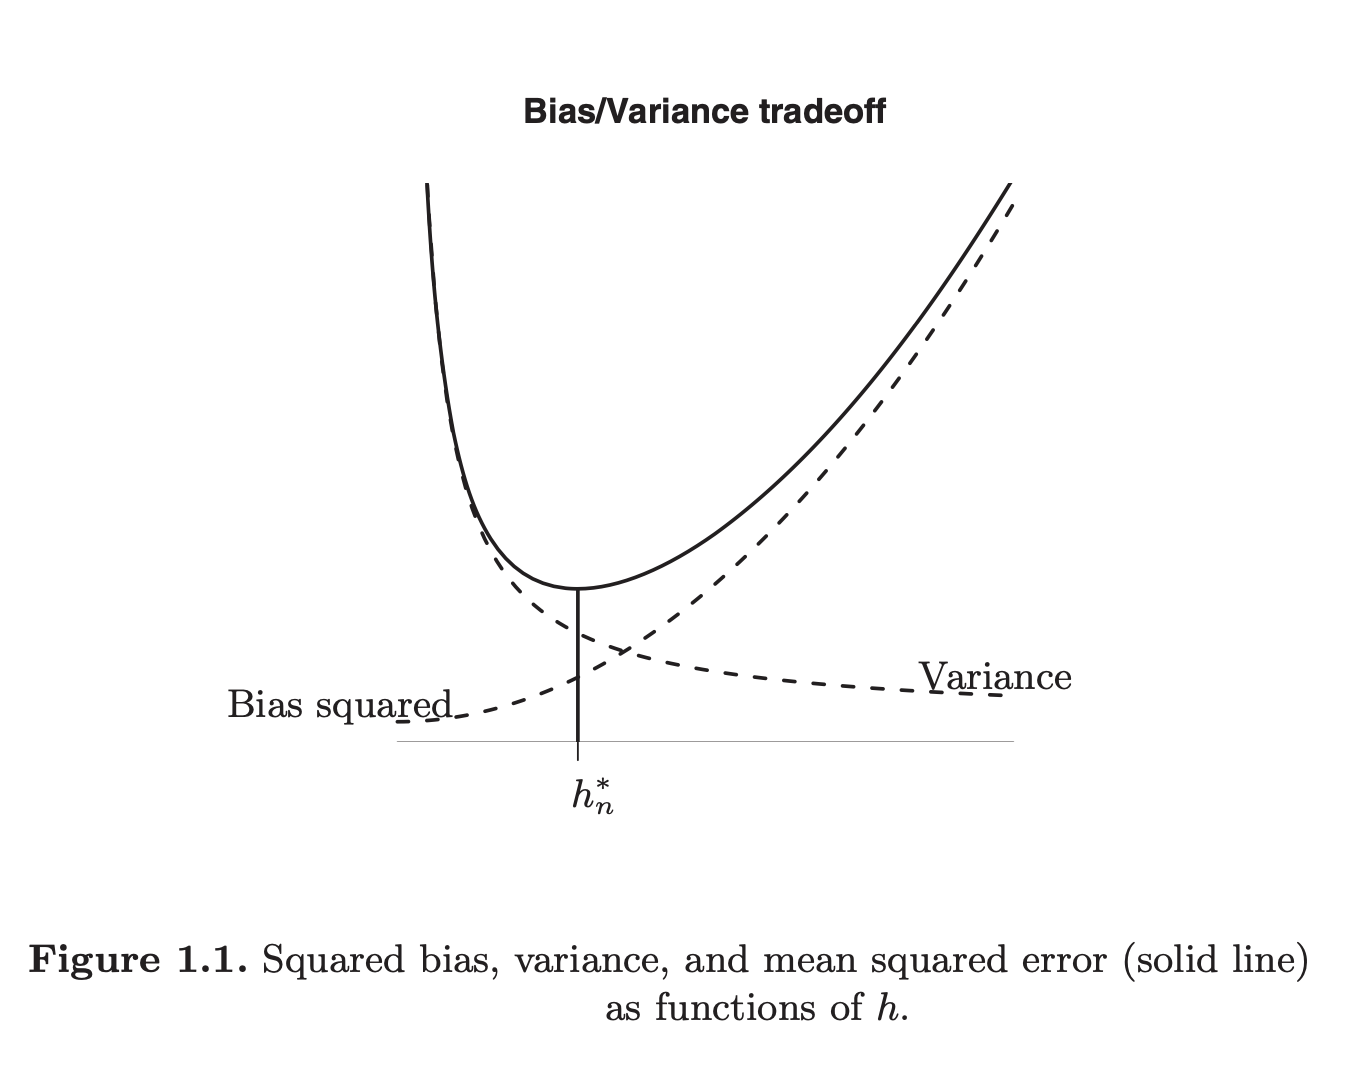
\includegraphics[width=0.8\textwidth]{trade_off_nonparametrics.png} % Replace with the actual path to your PNG file
    \caption{Squared bias, variance, and mean squared error (solid line) as functions of $h$.}
    \label{fig:tradeoff}
\end{figure}

Figure \ref{fig:smoothing_graphs} illustrates three key scenarios in kernel density estimation:
\begin{figure}[h]
    \centering
    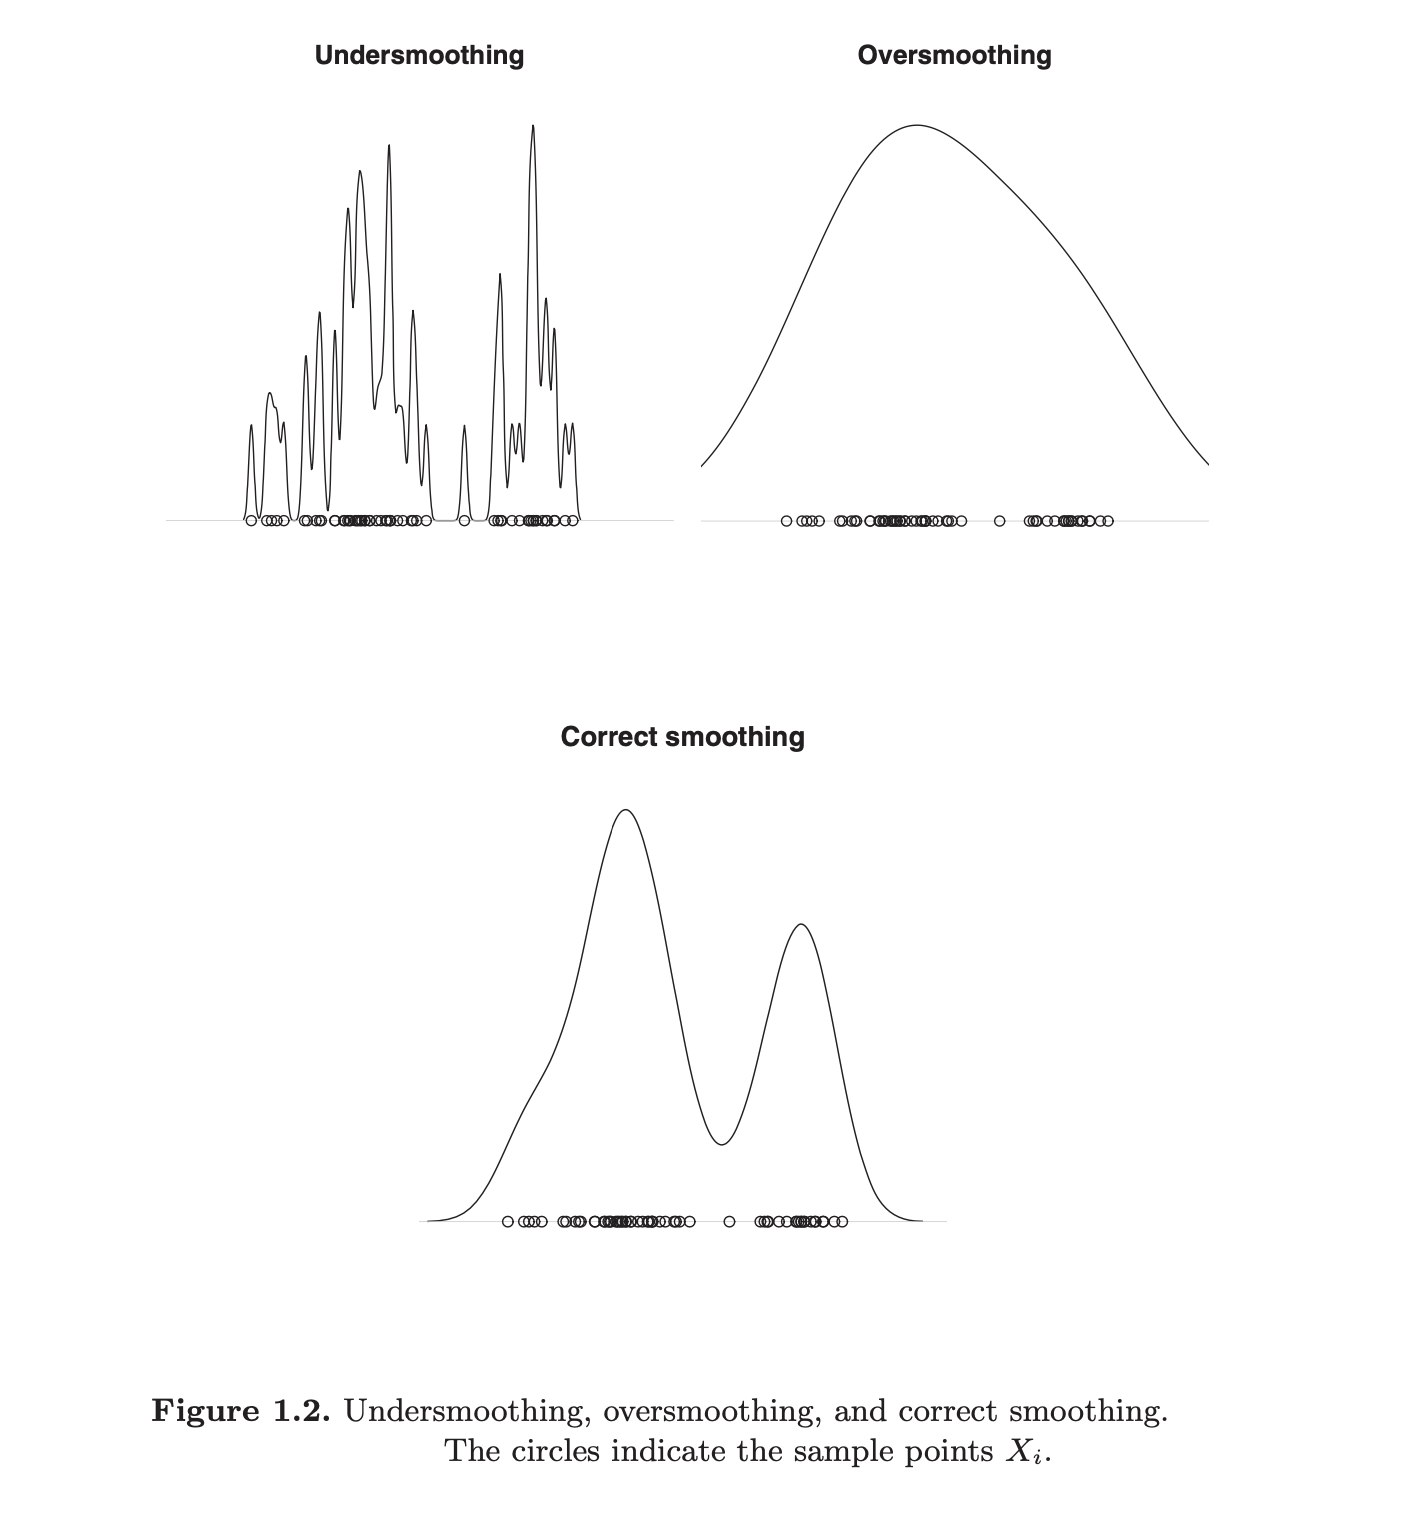
\includegraphics[width=0.8\textwidth]{graphs_1_nonparametrics.png} % Replace with the actual path to your PNG file
    \caption{Undersmoothing, oversmoothing, and correct smoothing. The circles indicate the sample points $X_i$.}
    \label{fig:smoothing_graphs}
\end{figure}

\begin{itemize}
    \item \textbf{Undersmoothing:} The bandwidth $h$ is too small, resulting in a noisy estimate that overfits the sample points. This leads to high variance.
    \item \textbf{Oversmoothing:} The bandwidth $h$ is too large, causing the estimator to oversimplify the density and miss important features such as modes. This leads to high bias.
    \item \textbf{Correct smoothing:} The bandwidth $h$ is chosen optimally, balancing the trade-off between bias and variance. The estimate captures the essential structure of the density.
\end{itemize}


The minimum with respect to \( h \) of the right-hand side of the MSE bound is attained at:
\[
    h_n^* = \left( \frac{3C_2}{2(\beta - 1)C_1^2} \right)^{\frac{1}{2\beta + 1}} n^{-\frac{1}{2\beta + 1}}.
\]
This differs from the result in the book, which presents:
\[
    h_n^* = \left( \frac{C_1}{2\beta C_2} \right)^{\frac{1}{2\beta+1}} n^{-\frac{1}{2\beta+1}}.
\]
\footnote{This is taken from the book, but we achieve different results because we are analyzing the derivative of the Kernel function.}

However, it is important to note that the \textit{rate of convergence} remains the same in both cases. Specifically, the MSE is given by:
\[
    \text{MSE}(x_0) = O\left(n^{-\frac{2\beta}{2\beta+1}}\right), \quad n \to \infty,
\]
uniformly in \( x_0 \).
\begin{theorem}
    Assume that condition (1.5) holds and the assumptions of Proposition 1.2 are satisfied. Fix $\alpha > 0$ and take $h = cn^{-\frac{1}{2\beta+1}}$. Then for $n \geq 1$, the kernel estimator $p_n$ satisfies:
    \[
        \sup_{x_0 \in \mathbb{R}} \sup_{p \in P(\beta, L)} \mathbb{E}_p\left[(p_n(x_0) - p(x_0))^2\right] \leq C n^{-\frac{2\beta}{2\beta+1}},
    \]
    where $C > 0$ is a constant depending only on $\beta$, $L$, $\alpha$, and on the kernel $K$.
\end{theorem}

\begin{proof} Using previous equation and bounding the supremum norm of the kernel density estimate
    \[
    \sup_{x \in \mathbb{R}, p \in P(\beta, L)} |p(x)| \leq p_{\max},
\]
where $p_{\max}$ is derived from boundedness properties of the kernel $K$ and its derivatives
\end{proof}


\subsubsection{Some definitions from class 6}
These are definitions and theorems that were not used in the seminar. Most of the theorems, definitions and proofs given in class 6 were given by the great and informative TD so I omit their repetition. 
\begin{proposition}
    Let \(f(x)\in \prob(\beta, l)\). With \(\beta>0\) and k of order \(L>0\) and \(l=\lfloor \beta \rfloor\)\footnote{In this case, the floor function holds strictly.} such that \(\int_{\R}|\mu|^{\beta} k(\mu) d\mu <\infty\) Then \(\forall x \in \R\) and \(\forall h>0\) \(|f(x)|\leq C_{1}h^{\beta}\) where \(C_{1}:=\frac{L}{!}\int_{\R}|\mu|^{\beta} k(\mu) d\mu\)
\end{proposition}

\begin{theorem}
    Assume k satisfies the assumptions of the previous proposition and of proposition xx \footnote{\textbf{I need a way to keep track of citations...add labels, lazy boy}} and choose \(h=\alpha n^{-\frac{1}{2\beta + 1}}\) for some \(\alpha \geq 0\) then: 
    \[
        \sup_{x \in \mathbb{R}} \sup_{f(x) \in \prob(\beta , l)} \E \left[ \left(\hat{f}_{x}(x)-f_{x}(x)\right)^{2}\right] \leq C n^{\frac{-2\beta}{2\beta+1}} \]

    
\end{theorem}
Note that the more variables we have in the analysis the  worse it gets...unbounded...

\begin{remark}
    Note that the previous theorem can also be expressed as \[ 
    \sup_{\hat{f}_x} \sup_{f(x) \in \prob(\beta , l)} \E \left[ \left(\hat{f}_{x}(x)-f_{x}(x)\right)^{2}\right] \geq C n^{\frac{-2\beta}{2\beta+1}}
    \]
    It is optimal up to a constant: 


    \[
    \sup_{\hat{f}_x} \sup_{f(x) \in \prob(\beta , l)} \E \left[ \left(\hat{f}_{x}(x)-f_{x}(x)\right)^{2}\right] n^{\frac{2\beta}{2\beta+1}} > 0 
    \]
\end{remark}








\end{document}
